\section{Day 12: Quotient Topology Examples; Connectivity (Oct. 10, 2024)}
Outfit of the day! no rainbow hat :c
\begin{figure}[h]
    \centering
    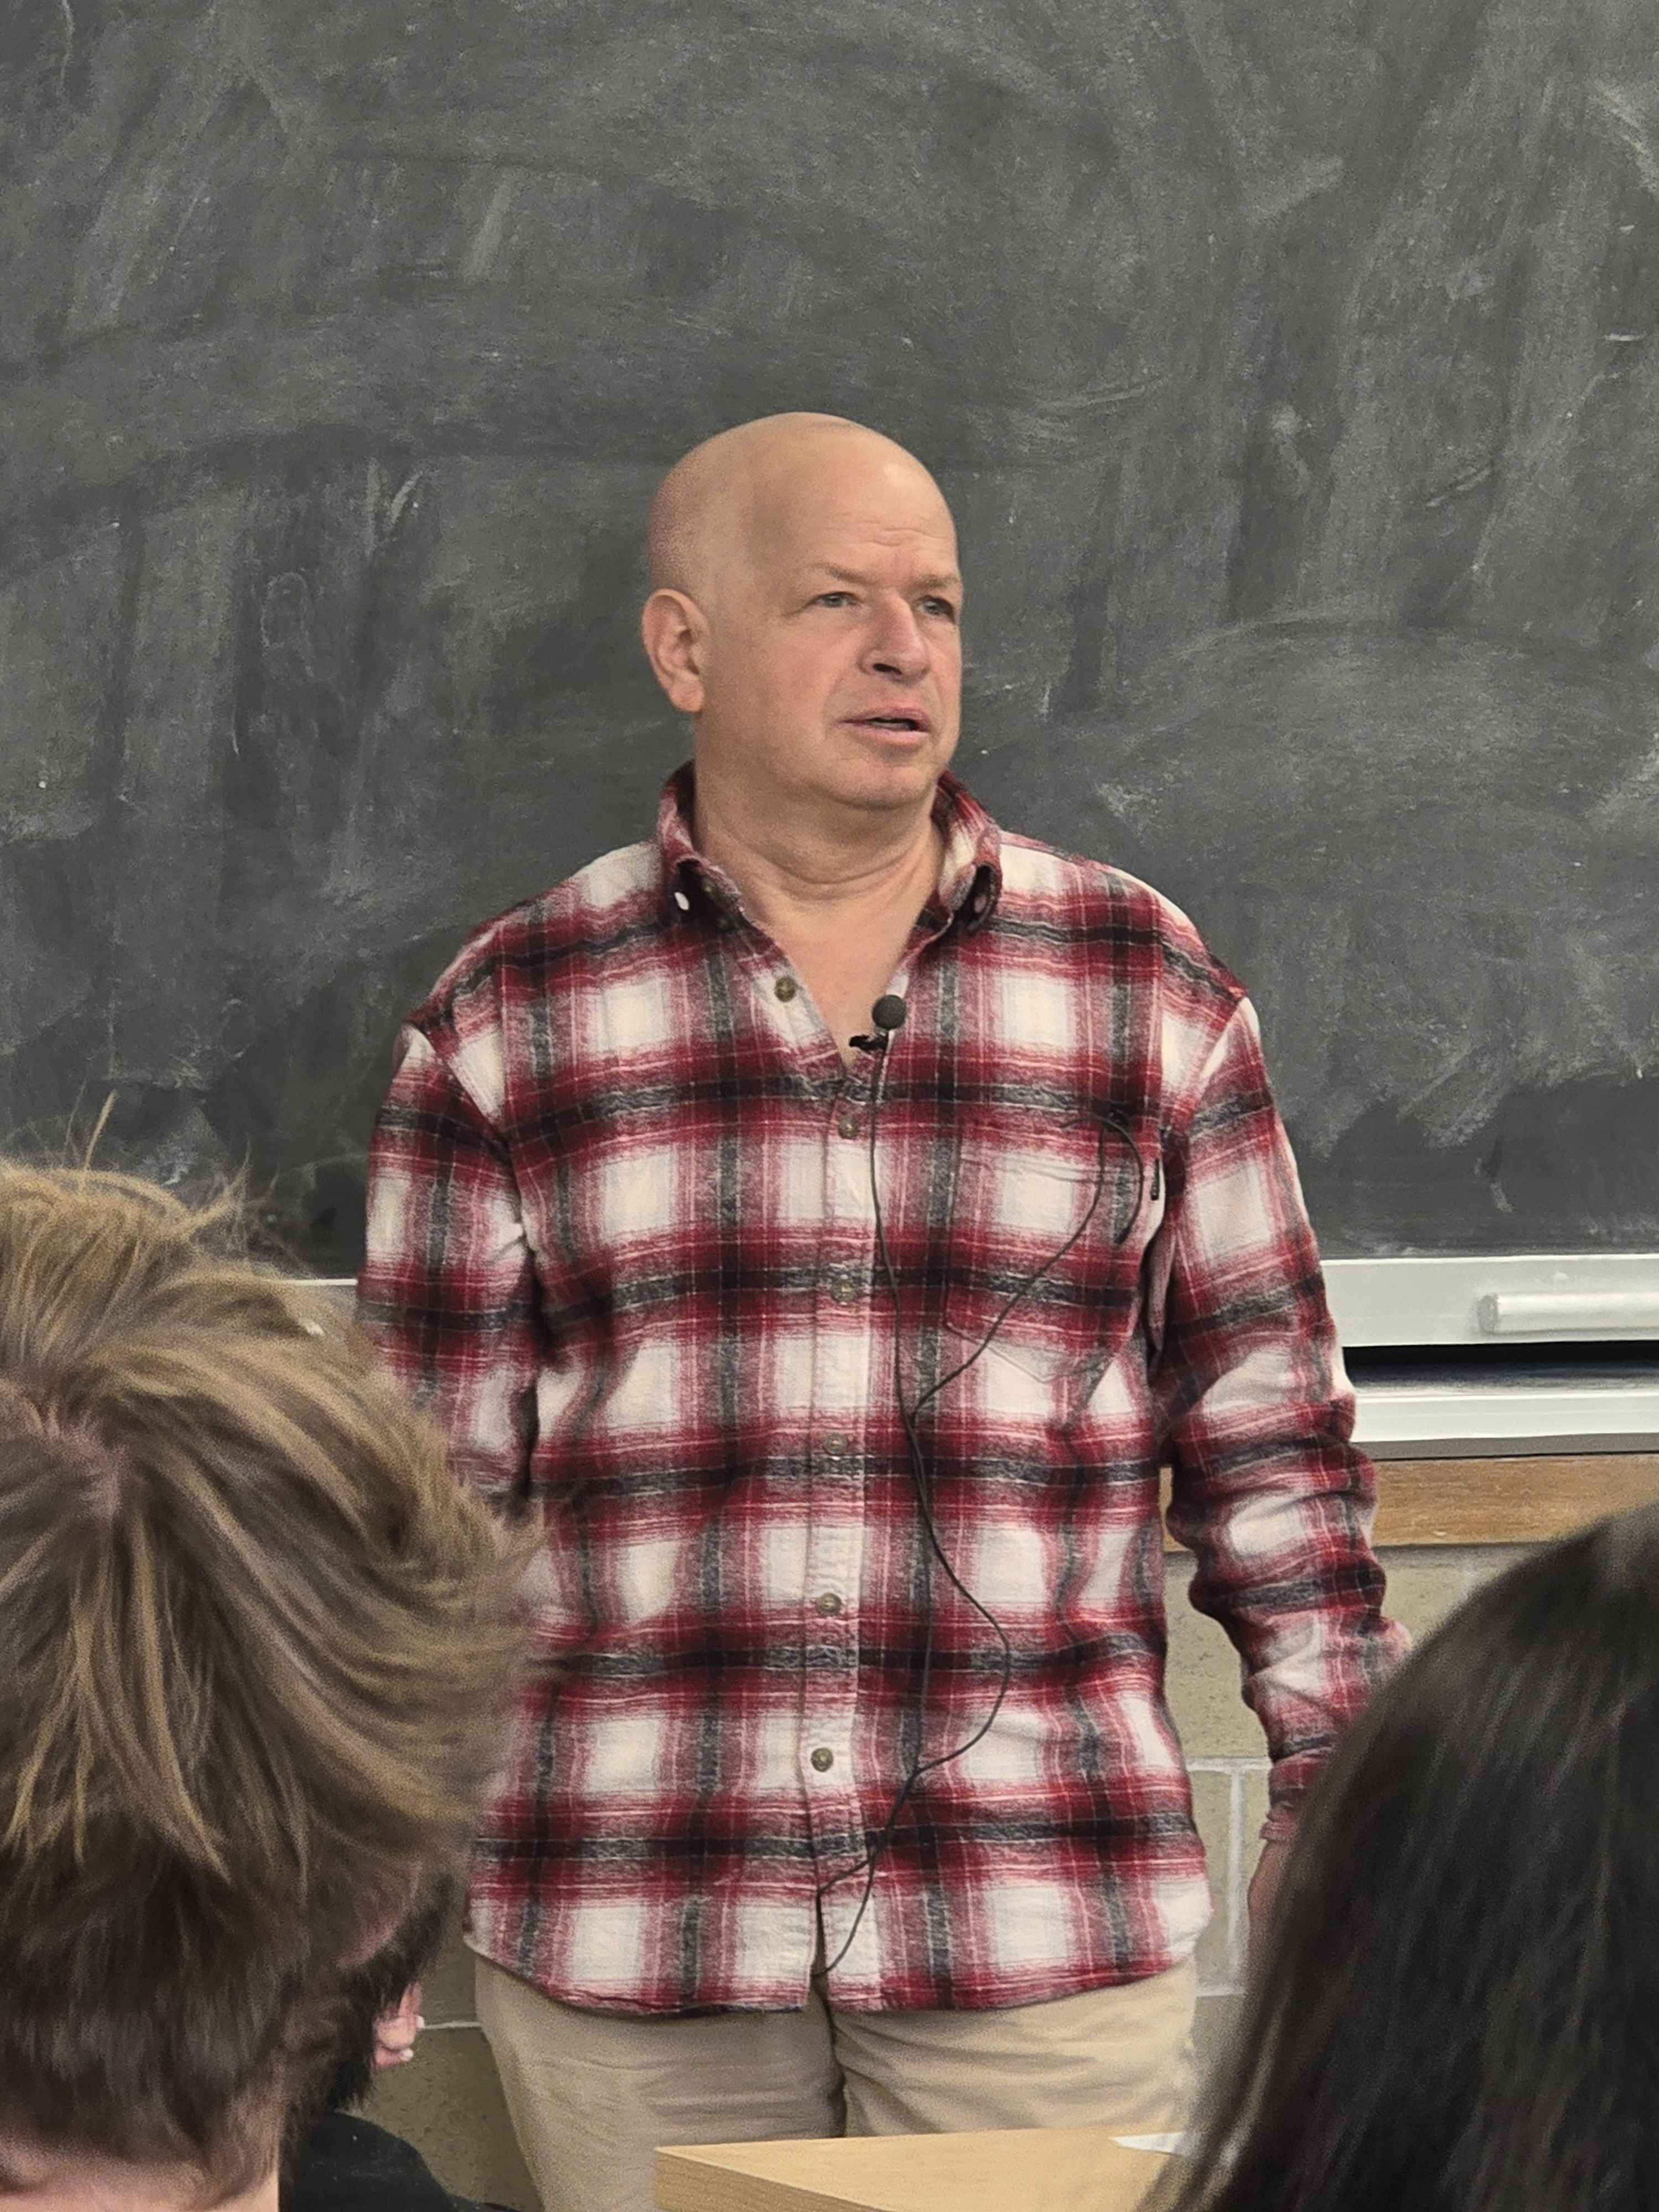
\includegraphics[scale=0.1]{MAT327 Notes/Dror Shirts/dror day 12 shirt.jpg}
\end{figure}

\noindent Recap! Given a surjection $\pi : X \to Y$ or a quotient map $\pi : X \to X/{\sim}$, seek a topology on $X/{\sim}$ such that
\begin{enumerate}[label=(\alph*)]
    \item $\pi : X \to X/{\sim}$ is continuous
    \item If $f : X/{\sim} \to Z$ is such that $f \circ \pi$ is continuous, then so is $f$.
\end{enumerate}
\begin{simplethm}
    Such a topology satisfying the above conditions exists, and is unique.
\end{simplethm}
\noindent We start with uniqueness. Observe the following diagram,
% https://q.uiver.app/#q=WzAsMyxbMSwwLCJYIl0sWzAsMSwiKFgvXFxzaW0pXzEiXSxbMiwxLCIoWC9cXHNpbSlfMiJdLFswLDEsIlxccGlfMSIsMl0sWzAsMiwiXFxwaV8yIl0sWzEsMiwiXFxpZCIsMl1d
\[\begin{tikzcd}
	& X \\
	{(X/{\sim})_1} && {(X/{\sim})_2}
	\arrow["{\pi_1}"', from=1-2, to=2-1]
	\arrow["{\pi_2}", from=1-2, to=2-3]
	\arrow["\id"', from=2-1, to=2-3]
\end{tikzcd}\]
Then the proof is similar to every other proof we have done before now; a continuous identity means they're the same. To check existence, let us have $\ST_{X/{\sim}} := \{V \subset X/{\sim} \mid \pi^{-1}(v) \in \ST_X\}$.

\newpage
\begin{simpleclaim}
    $\ST_{X/{\sim}}$ is indeed a topology on $X/{\sim}$ that satisfies (2).
\end{simpleclaim}
\noindent \textit{(Proof is left as an exercise)} \href{https://math.stackexchange.com/questions/1497863/why-is-the-quotient-topology-unique}{read this link mayb?}
\medskip\newline
We now go over some examples.
\begin{enumerate}[label=(\alph*)]
    \item Consider $S^1 = \bigslant{[0, 1]}{0 \sim 1} = \{x \sim x \mid x \in [0, 1]\} \cup \{0 \sim 1, 1 \sim 0\}$. Then this is equivalent to $(0, 1) \cup N$, where $N$ is a new point next to $0$ and $1$ (read: $N$ is a point connecting the endpoints of the interval $[0, 1]$ to ``join'' it into the circle $S^1$).
    \item $X = \bigslant{[0, 1] \times [0, 1]}{(0, y) \sim (1, y)}$ for all $y \in [0, 1]$. Here, imagine a unit square; we are identifying its vertical edges as identical; this is similar to (a), except we have a square instead of a unit interval. Thus, we see $X$ is basically a cylinder.
    \item $X = \bigslant{[0, 1] \times [0, 1]}{(0, y) \sim (1, 1-y)}$ is a M\"obius band.
    \item $X = \bigslant{[0, 1] \times [0, 1]}{\substack{(0, y) \sim (1, y) \\ (x, 0) \sim (x, 1)}}$ is a torus.
    \item $X = \bigslant{[0, 1] \times [0, 1]}{\substack{(0, y) \sim (1, y) \\ (x, 0) \sim (1 - x, 1)}}$ is a Klein bottle.
    \item $\RR\PP^2$ or $\PP_2(\RR)$ (the real projective space, \href{https://www.mfo.de/about-the-institute/history/boy-surface}{here}), given by $\bigslant{[0, 1] \times [0, 1]}{\substack{(0, y) \sim (1, 1 - y) \\ (x, 0) \sim (1 - x, 1)}}$ cannot be embedded in $\RR^3$;   
    \item octagon type shit
    \item Let us consider vectors $v$ as having magnitude and direction; we may write them as $\abs{v} \in \RR$, and the direction belongs in $\mathrm{dir}(v) = \bigslant{v}{\substack{v_1 \sim \alpha v_2 \\ \alpha > 0}}$.
\end{enumerate}